\documentclass[english]{article}
\usepackage[T1]{fontenc}
\usepackage[utf8]{inputenc}
\usepackage{csquotes}
\usepackage[colorlinks=true, citecolor = blue]{hyperref}      % hyperlinks
\usepackage{multirow, amssymb, amsmath, graphicx, arydshln, url}
\usepackage[T1]{fontenc}
\usepackage{natbib}

\title{Supporting Information for ``Modelling publication bias and \textit{p}-hacking''\\ by Jonas Moss and Riccardo De Bin}

\author{}

\date{}

\begin{document}

\maketitle


\section*{Web Appendix A}

Recall that a density $f(x;\theta)$ is identified if $f(x;\theta_{1})=f(x;\theta_{2})$
for all $x$ implies that $\theta_{1}=\theta_{2}.$ Call a density
$f(x;\theta)$ \textit{strongly identified} if $f(x;\theta_{1})/f(x;\theta_{2})$
being constant for all $x$ in an open interval $I$ implies that
$\theta_{1}=\theta_{2}$.
\paragraph{Proposition A.}\label{prop:identified}

Let $f(x;\theta)$ be a family of densities on $\mathbb{R}$, $-\infty=a_{1}<a_{2}<\ldots<a_{k+1}=\infty$
a sequence of cutoffs, and $f_{[a_{i},a_{i+1}]}(x;\theta)$ the density
$f$ truncated to $[a_{i},a_{i+1}]$. Let $\lambda_{i},k=1,\ldots k$
be positive numbers satisfying $\sum_{i=1}^{k}\lambda_{i}=1$. Then
the mixture
\[
g(x;\lambda,\theta)=\sum_{i=1}^{k}\lambda_{i}f_{[a_{i},a_{i+1})}(x;\theta)
\]
is identified in $(\lambda,\theta)$ if $f(x;\theta)$ is strongly
identified in $\theta$.

\paragraph{Proof.}
Assume that $g(x;\lambda_{1},\theta_{1})=g(x;\lambda_{2},\theta_{2})$.
Then $$\lambda_{1i}f_{[a_{i},a_{i+1}]}(x;\theta_{1})=\lambda_{2i}f_{[a_{i},a_{i+1}]}(x;\theta_{2})$$
for all $i$, thus
\[
\frac{\lambda_{1i}}{\lambda_{2i}}=\frac{f_{[a_{i},a_{i+1})}(x;\theta_{1})}{f_{[a_{i},a_{i+1})}(x;\theta_{2})}.
\]
This implies that $f(x;\theta_{1})/f(x;\theta_{2})$ is constant for
$x\in[a_{i},a_{i+1}]$. But since $f(x;\theta)$ is strongly identifiable,
$\theta_{1}=\theta_{2}$, and, consequently, $\lambda_1 = \lambda_2$.


If $f(x;\theta)$ is real analytic and nowhere zero, $f(x;\theta_{1})/f(x;\theta_{2})$
is also real analytic and nowhere zero. By the Identity Theorem \citep[Corollary 1.2.6]{Krantz2002-bt}, if the ratio
$f(x;\theta_{1})/f(x;\theta_{2})$ is constant on some interval $I$,
then $f(x;\theta_{1})/f(x;\theta_{2})$ is constant everywhere, hence
$f(x;\theta_{1})=f(x;\theta_{2})$ everywhere. Thus a family of real
analytic nowhere zero densities is identified if and only if it is
strongly identified. Every exponential family of densities on the form
\[
f(x;\theta)=h(x)\exp(\eta(\theta)^{T}T(x)-A(\theta))
\]
satisfies this property, provided only that $h$ is nowhere zero real analytic
and $T$ is real analytic. In particular, the normal family satisfies
the properties.

Not every density is strongly identified. For instance, mixtures of uniforms are not strongly identified. And indeed, Proposition A fails when $f$ is a mixture of uniforms.

%\paragraph{Proof of Proposition 1}

%We only need to show that $q_{H}(x)$ integrates to $1$.
%\begin{eqnarray*}
%\int f_{H}(x)dx & = & \int\frac{p(s=1)}{p(s=1\mid y_{H^{c}})}p(y)dx\\
% & = & \int\frac{p(s=1\mid y_{H},y_{H^{c}})}{p(s=1\mid y_{H^{c}})}p(y_{H^{c}}\mid y_{H})p(y_{H})dy_{H^{c}}dy_{H}\\
% & = & \int\frac{p(s=1\mid y_{H^{c}})}{p(s=1\mid y_{H^{c}})})p(y_{H^{c}})dy_{H^{c}})\\
% & = & 1
%\end{eqnarray*}




\section*{Web Appendix B}

As mentioned in Section 2, any \textit{p}-hacking model can be written on the form of a selection model. Observe that
\begin{eqnarray*}
\int_{[0,1]}f_\alpha^{\star}(x_{i}\mid\theta_{i},\eta_{i}, u)d\omega(\alpha) & = & \int_{[0,1]}f(x_{i}\mid\theta_{i})P(u\in\left[0,\alpha\right]\mid\theta_{i},\eta_{i})^{-1}d\omega(\alpha)\\
 & = & f(x_{i}\mid\theta_{i})\int_{[0,u]}P(u\in\left[0,\alpha\right]\mid\theta_{i},\eta_{i})^{-1}d\omega(\alpha).
\end{eqnarray*}
where $f_\alpha^{\star}$ is the density $f^{\star}$ truncated so that the \textit{p}-value $u\in\left[0,\alpha\right]$. This is a publication bias model if $$h(u)=\int_{[0,u]}P(u\in\left[0,\alpha\right]\mid\theta_{i},\eta_{i})^{-1}d\omega(\alpha)$$ is bounded for each $u$ and $h(u)$ is independent of $\theta_{i},\eta_{i}$. While $h(u)$ can be bounded, it is typically dependent of $\theta_{i},\eta_{i}$, with the fixed effect model under complete selection for significance being a notable exception.

On the other hand, any selection model $f(x_{i};\theta_{i},\eta_{i})\rho(u)$ with $I =\int f(x;\theta_{i},\eta_{i})\rho(u)du<\infty$ can be written as a mixture model. For then there is a finite measure $d\omega(\alpha;\theta_{i},\eta_{i})$ satisfying 
\[
\rho(u)=\int_{[0,u]}\frac{1}{P(u\in\left[0,\alpha\right]\mid\theta,\eta)}d\omega(\alpha;\theta_{i},\eta_{i})
\]
Just take $d\omega(\alpha;\theta_{i},\eta_{i})=d\rho(\alpha)P(u\in\left[0,\alpha\right]\mid\theta_{i},\eta_{i})$, where $d\rho(\alpha)$ is defined by $\int_{0}^{u}d\rho(\alpha)=\rho(u)$. The size of the measure is
\begin{eqnarray*}
\int_{0}^{1}d\omega(\alpha;\theta_{i},\eta_{i}) & = & \int_{0}^{1}P(u\in\left[0,\alpha\right]\mid\theta_{i},\eta_{i})d\rho(\alpha)\\
 & = & \int_{0}^{1}f(u;\theta_{i},\eta_{i})\int_{0}^{u}d\rho(\alpha)du\\
 & = & I
\end{eqnarray*}
Hence $I_{\theta,\eta}d\omega'(\alpha;\theta_{i},\eta_{i})$ is a probability measure. This probability measure makes 
\[
I^{-1}f(x_{i};\theta_{i},\eta_{i})\rho(u)=\int_{[0,1]}f_\alpha(x_{i};\theta_{i},\eta_{i})d\omega'(\alpha)
\]
as can be seen by the following computation,
\begin{eqnarray*}
I^{-1}f(x_{i};\theta_{i},\eta_{i})\rho(u) & = & I^{-1}\int_{[0,u]}\frac{f(x_{i};\theta_{i},\eta_{i})}{P(u\in\left[0,\alpha\right]\mid\theta_{i},\eta_{i})}d\omega(\alpha)\\
 & = & I^{-1}\int_{[0,1]}\frac{f(x_{i};\theta,\eta)1_{\left[0,\alpha\right]}(u)}{P(u\in\left[0,\alpha\right]\mid\theta_{i},\eta_{i})}d\omega(\alpha)\\
 & = & I^{-1}\int_{[0,1]}f_\alpha(x_{i};\theta_{i},\eta_{i})d\omega(\alpha)\\
 & = & \int_{[0,1]}f_\alpha(x;\theta_{i},\eta_{i})d\omega'(\alpha)
\end{eqnarray*}

Proposition 1 shows the form of the one-sided normal step function selection probability publication bias model when it is written as a mixture model of the form (5). But most such mixture models are not true \textit{p}-hacking models, as the mixing probabilities $\pi_{i}^{\star}$ depend on $\theta$. There is no way for the \textit{p}-hacker to know
$\theta$, so we cannot regard the publication bias model as a \textit{p}-hacking model.




% \section*{Web Appendix C}

% \subsubsection*{Graphical representation of selection models}

% It is handy to visualize selection models and their selection sets using directed acyclic graphs. To this end recall that a Bayesian network is a directed acyclic graph $G$ together with a probability density $p$ satisfying the property that $p(x)=\prod_{v\in V(G)}p(x_{v}\mid x_{\textrm{pa}(v)})$, where $V(G)$ is the set of vertices in $G$ and $x_{\textrm{pa}(v)}$ are the parents of $x_{v}$ in $G$ \citep{Pearl2014}. Transforming a Bayesian network for $p$ into a Bayesian network for $q_{H}$ is easy, just add the following to $G$: (i) The selection variable vertex $s$, and (ii) arrows $x$ to $s$ for each $x$ that $s$ depends on. Then
% \begin{equation}
% q_{H}(x\mid s=1)=\frac{p(s=1\mid x_{\textrm{pa}(s)})}{p(s=1\mid H^{c})}\prod_{v\in V(G)}p(x_{v}\mid x_{\textrm{pa}(v)})\label{eq:DAG, selection model}.
% \end{equation}

% To visualize the selection set $H$, start by drawing a dashed plate around the vertices in $H$. In plate notation \citep{buntine1994operations}, a solid plate represents variables that are sampled together. The dashed plate does almost the same, for recall that $H$ contains all the elements that are sampled together until $s=1$. The semantic difference between a dashed and a solid plate is that every sample in a solid plate is observed, but only one of potentially many samples in a dashed plate is observed. The following bare-bones example should make things clear.

% Figure \ref{fig:Plate notation, simple example} displays the directed acyclic graphs of $p$ and the selection models when $H = \emptyset$, $H=\left\{ x,\theta\right\}$, and $H=\left\{ x\right\}$, respectively. The marginal distribution of $\theta$ is not the same for $H=\left\{ x\right\}$ and $H=\left\{ x,\theta\right\} $, as $q_{\left\{ x,\theta\right\} }(\theta) = p(\theta)\frac{p(s=1\mid\theta)}{p(s=1)}$ and $q_{x}(\theta) = \int\frac{p(s=1\mid x)}{p(s=1\mid\theta)}p(x,\theta)dx=p(\theta)$, i.e., it is affected by the selection mechanism $s$.

% \subsubsection*{Example}\label{exa:Marginal density of theta}
% Let $p(x,\theta)=p(x\mid\theta)p(\theta)$ be a density and $s$ be a function of $x$ only, so that $p(s=1\mid x,\theta)=p(s=1\mid x)$.
% The possible selection models are
% \begin{eqnarray*}
% q_{\emptyset}(x,\theta) = q_{\theta}(x,\theta) & = & p(x,\theta)\\
% q_{(x,\theta)}(x,\theta) & = & \frac{p(s=1\mid x)}{p(s=1)}p(x,\theta)\\
% q_{x}(x,\theta) & = & \frac{p(s=1\mid x)}{p(s=1\mid\theta)}p(x,\theta)
% \end{eqnarray*}

% \begin{figure}
% \begin{center}     
%  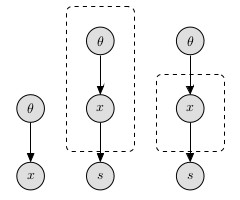
\includegraphics{plots/figure_A.jpg}
% \end{center}
% \caption{\label{fig:Plate notation, simple example} Three simple selection models. {\bf (left)} the original $p(x,\theta)$; {\bf (middle)} the model $q_{\left\{ x,\theta\right\} }$, where $\theta$ and $x$ are
% sampled together until $s=1$; {\bf (right)} the model $q_{x}$, where only $x$ is sampled until $s=1$.}
% \end{figure}

% Let $f(x,\theta\mid\eta)=f(x\mid\theta,\eta)p(\theta)$ be the joint density of a random effects meta-analysis, where $x$ is the effect size, $\theta$ is the study-specific parameter of interest, and $\eta$ is a study-specific nuisance parameter such as the sample size of the study. The left plot of Figure \ref{fig:Plate notation, simple example} is a visualization of $f(x,\theta)$. If we have more than one study to analyse, we will have to work with product density $\prod_{i=1}^{n}f(x_{i},\theta_{i}\mid\eta_{i})$ instead of the stand-alone density $f(x,\theta\mid\eta)$. This is visualised in the middle plot of Figure \ref{fig:Plate notation, simple example}  by drawing a solid plate around the pair $(x,\theta)$. When we are dealing with a fixed effects meta-analysis, in which $\theta$ is fixed, the plate should be drawn around $x$ only (Figure \ref{fig:Plate notation, simple example}, right graph). 

% \subsubsection*{Graphical representation of the publication bias and $p$-hacking models}

% To visualize selection models based on \textit{p}-values, we must make some modifications to the original graph: (i) Add the \textit{p}-value node $u$; (ii) Add an arrow from $x$ to $u$; (iii) Since the \textit{p}-value $u$ usually depends on more information than just $x$, such as the standard deviation of $x$, add an arrow from $\eta$ (which represents the extra information) to $u$ as well; (iv) Add the selection node $s$ and an arrow from $u$ to $s$. If $u$ is the only parent of $s$, we are dealing with selection models only based on \textit{p}-values.

% The placement of dashed and solid plates depends on which model we want to use. The idea behind the publication bias model is that a completely new study is done whenever the last one failed to be published. This implies that $\theta$ and $x$ are sampled together. The left plot of Figure \ref{fig:Plate notation, publication bias and p-hacking} shows the direct acyclic graph of the normal publication bias model defined in Proposition 3 in the main text. In this particular case, $\eta$ corresponds to $\sigma$, the standard deviation. Moreover, $u$ is a \textit{p}-value, $\theta_{0}$ is the mean of the effect size distribution, $\tau$ is the standard deviation of the effect size distribution, and $\rho$ is the selection probability function. The variable $Z$ lives on the unit interval, and encodes the editor's decision to publish: If the observed \textit{p}-value is less than $Z$, the study is published. Importantly, $Z$ is placed inside the selection set because a new \textit{p}-value cut-off decision is made for each study received. Since $x$ and $\theta$ are sampled together, the selection mechanism modifies $p(\theta)$.%, as can be seen in the example \ref{exa:Publication bias, theta distribution} here below.

% In the \textit{p}-hacking scenario, the \textit{p}-hacker will hack his study all the way to significance, regardless of $\theta$. This means that $\theta$ and $x$ are sampled separately and $\theta$ must be placed outside the selection set. Moreover, the decision of how much to \textit{p}-hack is not reevaluated at each attempt. Consequently, the random variable that controls the \textit{p}-hacking decisions, analogously to the publication bias model, $Z$, is also placed outside the selection graph. This is the case, for example, of an author who decides to \textit{p}-hack to level $\alpha$ ($Z = \alpha$): he acts on $x$ to obtain the desired \textit{p}-value, whatever the sampled $\theta$ is. The graphical representation of this model is shown in the right plot of Figure \ref{fig:Plate notation, publication bias and p-hacking}. Since $x$ and $\theta$ are not sampled together, the selection mechanism does not modify $p(\theta)$.

% \begin{figure}
% \begin{center}
% 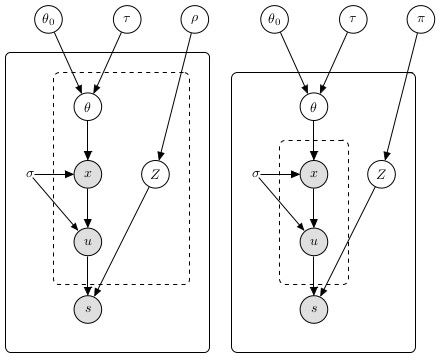
\includegraphics{plots/figure_B.jpg}
% \end{center}
% \caption{\label{fig:Plate notation, publication bias and p-hacking} Directed acyclic graphs for: {\bf (left)}
% the publication bias model; {\bf (right)} the \textit{p}-hacking model. The dashed plates enclose the selection sets and the the solid plates enclose variables that are repeated together.}
% \end{figure}

% \section*{Web Appendix C}


\bibliographystyle{biom}
\bibliography{main.bib}

\end{document}